\section{Development}

\subsection{Used frameworks and libraries}
ReceiptBudget is a web application written in Python, using the Django framework  \cite{django}. Django is a high-level framework for doing rapid Web development in Python. It provides an out-of-the-box administration interface, an object-relational mapper that allows models to be written in Python, without any SQL code, a URL routing framework and a powerful templating system.

The maps of the dashboard were developed using the Google Maps API v3 \cite{gmapsjs}, which provides the mapping service for the heatmaps. The d3.js libray \cite{bostock2011d3} is the backbone of the dashboard. It provides a declarative way to view data in all kinds of visual ways and to make them interactive. The dc.js is a visualization framework built on top of d3.js which provides several standard graphical views, such as bar charts, pies, line charts. To provide a way to filter and drill down the data the crossfilter Javascript is used, which provides fast multidimensional filtering for coordinated views, allowing the user to select a subset of the data in one chart and updating the other charts to only include data from that subset. 

For the processing of the image the OpenCV libray is used, with its Python bindings. The scikit-learn library \cite{pedregosa2011scikit} is used for the random forest and SVM implementations, while the neural networks are used from the pylearn2 library \cite{goodfellow2013pylearn2}. 
\subsection{Requirements Analysis}
The application needs to support multiple users. New users can create an account by registering. After that they can import a CSV file that was exported from other finance management software. 

An authenticated user can then start inserting his expenses. He has three ways to do this. The first one is to take a picture of the receipt using a webcam. The second is to upload a photo containg a receipt from his harddrive. The last option is to enter the details of the receipt manually. 

In the dashboard, the user has three views where he can visualize his expenses. He can see a heat map of all his expenses. Another view is a dynamic heat map that shows the progression of his expenses day by day. The last view is the one which contains the interactive charts and graphs. Here the user can see detailed breakdowns of his expenses by day of week, shop, months and date range, hopefully noticing any negative spending patterns that can be cut down. 

If a users expenses for the past week are over the average weekly expenses, they will receive a visual warning, reminding them to be careful with what they spend their money on. This warning comes as a bright colored bar at the top of the screen, with the intensity of the color depending on how much the user stepped over the normal expense range. 
\subsection{Design}
The default administration provided by the Django framework is customized to make it fit together with the rest of the website, both from a UI perspective and from a security point of view. By default, the administration interface shows every existent object from the database. This is changed so that it shows only the expenses that belong to the current user. These changes are done by subclassing the default admin classes and registering the child classes instead of them. The corresponding UML diagram can be seen in Figure \ref{fig:admin_classes}.
\begin{figure}[h!]
\begin{center}
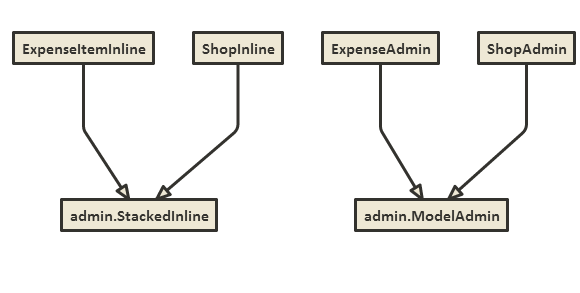
\includegraphics[width=\linewidth]{img/admin_classes.png}
\caption{\label{fig:admin_classes}
The classes used for the administration interface of the application}
\end{center}
\end{figure}

There are four entities that need to be stored in the database. One of them is a user entity, which is provided by the Django framework with everything it needs, including a profile, registration, password recovery and other security measures. 

The other entities are a \textbf{Shop}, where expenses can be made, an \textbf{Expense}, which has expense items, and \textbf{ExpenseItems}, which are the atomic elements of spending. 

Shops have a name, an address, a CUI and geographical coordinates. These are determined from the address via a geocoding service, such as the one offered by Google. The geographical coordinates are stored in the database, even though they are computable attributes because making the call to an external service is costly and because the number of calls that can be made per second is limited. Because of this, whenever a new shop is introduced, or when an existing shop is modified, a call is made to determine its location. This location is then used to plot on the heatmap.

Expenses have a date on which they were made and a user to whom they belong. They must have at least one Expense Item, but up to any number of them. They provide a property to calculate the total amount spent, by summing all the individual expenses. 

Expense items have a name and a price associated with them and represent the fundamental element where money is spent. They are individual items that can be bought. 

The UML diagram showing these classes can be seen in Figure \ref{fig:classes}.

\begin{figure}[h!]
\begin{center}
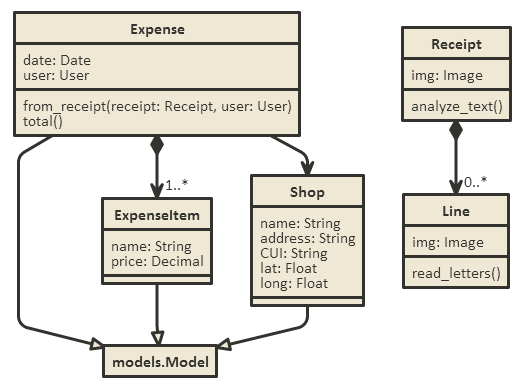
\includegraphics[width=\linewidth]{img/classes.png}
\caption{\label{fig:classes}
UML diagram of the classed used for the models and for the OCR engine}
\end{center}
\end{figure}

The OCR engine has two entities: receipts and lines. A receipt can have multiple lines. The receipt is responsible for cleaning up the input image, preprocessing it and finding the lines in it, which are then instantiated as separate objects which perform the actual process of character segmentation and recognition. After all the lines have finished recognizing, the receipt object can classify its lines and then it can return the properties of the receipt: date, shop, CUI, address, items, total. 

% \subsection{Implementation}
% mai trebuie asta?

\subsection{User Manual}
\label{sec:manual}

When a user comes to the ReceiptBudget website, he is presented with the main landing page, which can be seen in Figure \ref{fig:intro}. If he has an account, he can log in, if not he can create an account, using the form in Figure \ref{fig:register}, after which he is logged in automatically.

\begin{figure}[htdp]
\begin{center}
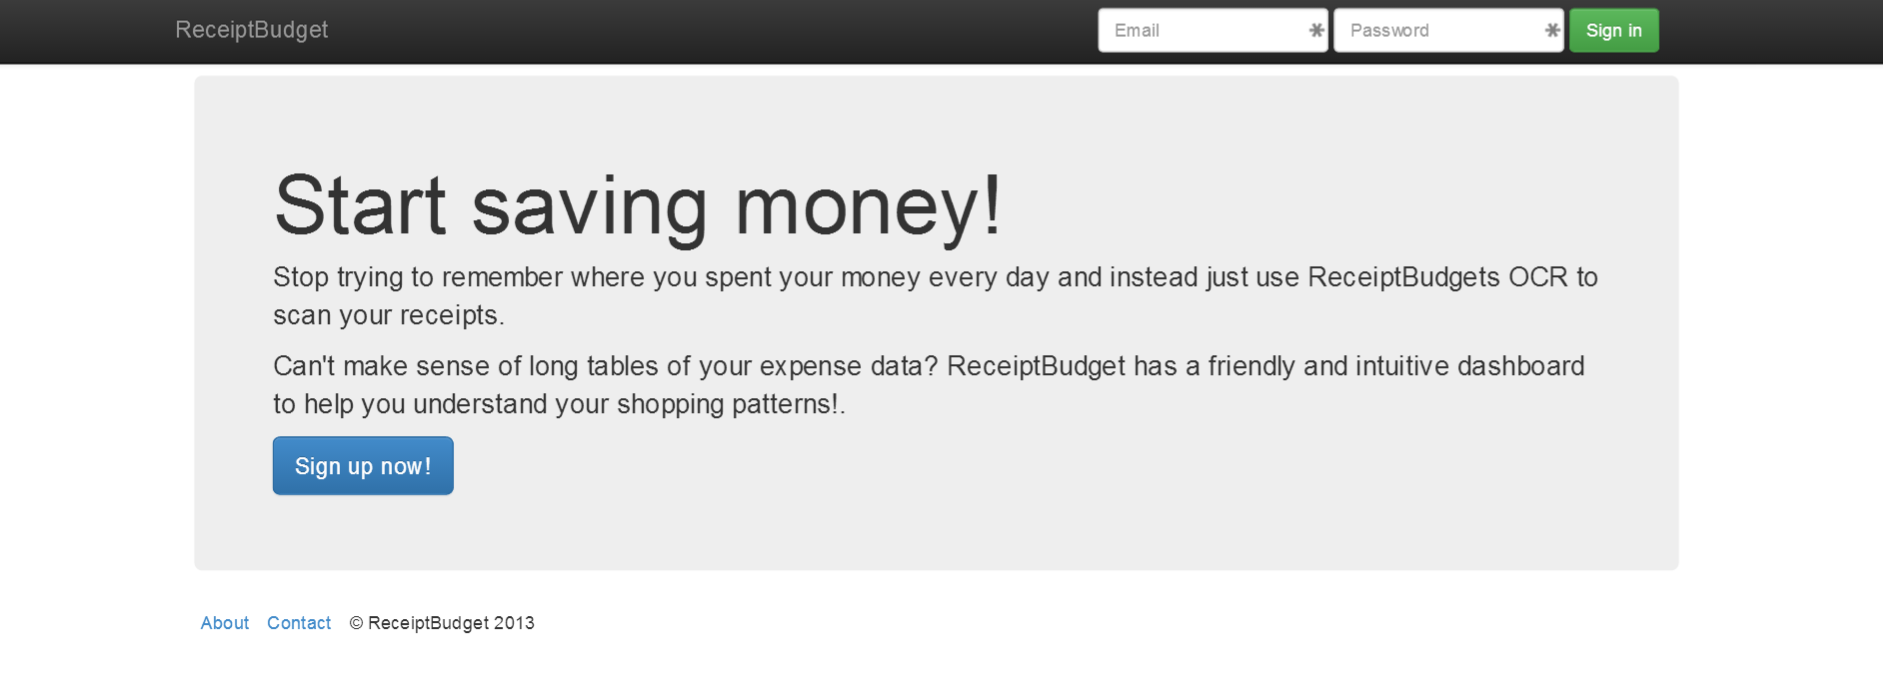
\includegraphics[width=\linewidth]{img/manual/intro.png}
\caption{\label{fig:intro}
The home page shown to a user who is not yet logged-in}
\end{center}
\end{figure}

\begin{figure}[htdp]
\begin{center}
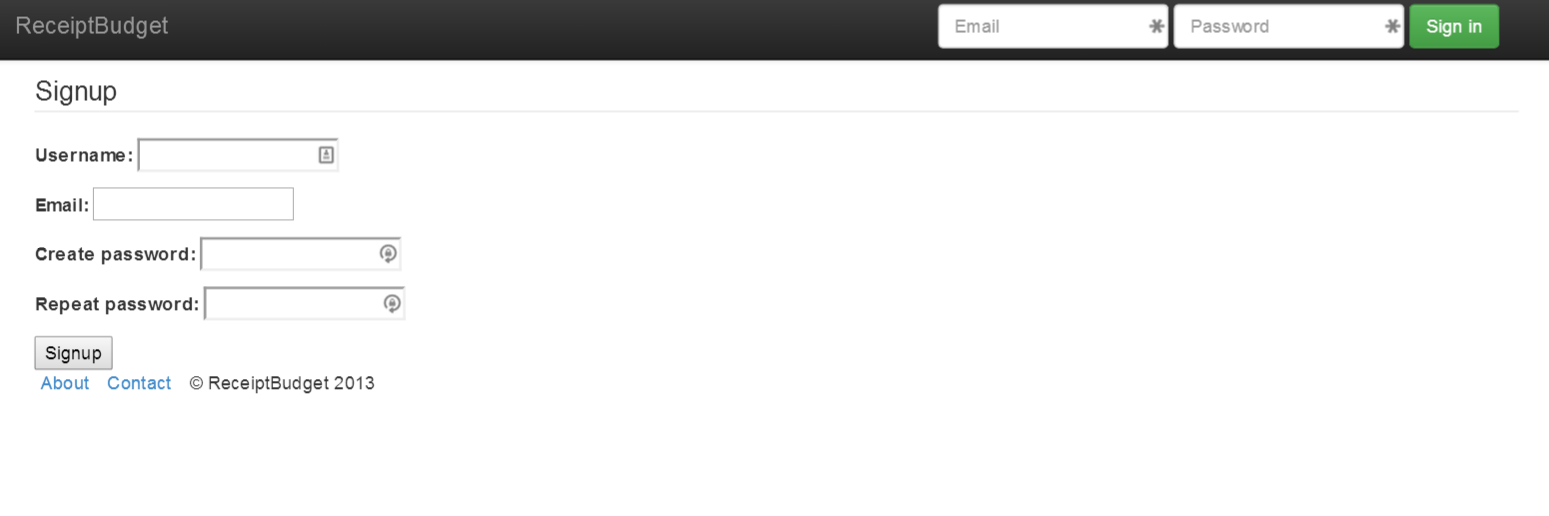
\includegraphics[width=\linewidth]{img/manual/register.png}
\caption{\label{fig:register}
The registration screen}
\end{center}
\end{figure}

After a user has logged in, he is presented with a list of his expenses, similar to the one in Figure \ref{fig:expense_list}. He can then choose to add a new expense, edit an existing one, view the dashboard or edit his user profile. 
\begin{figure}[htdp]
\begin{center}
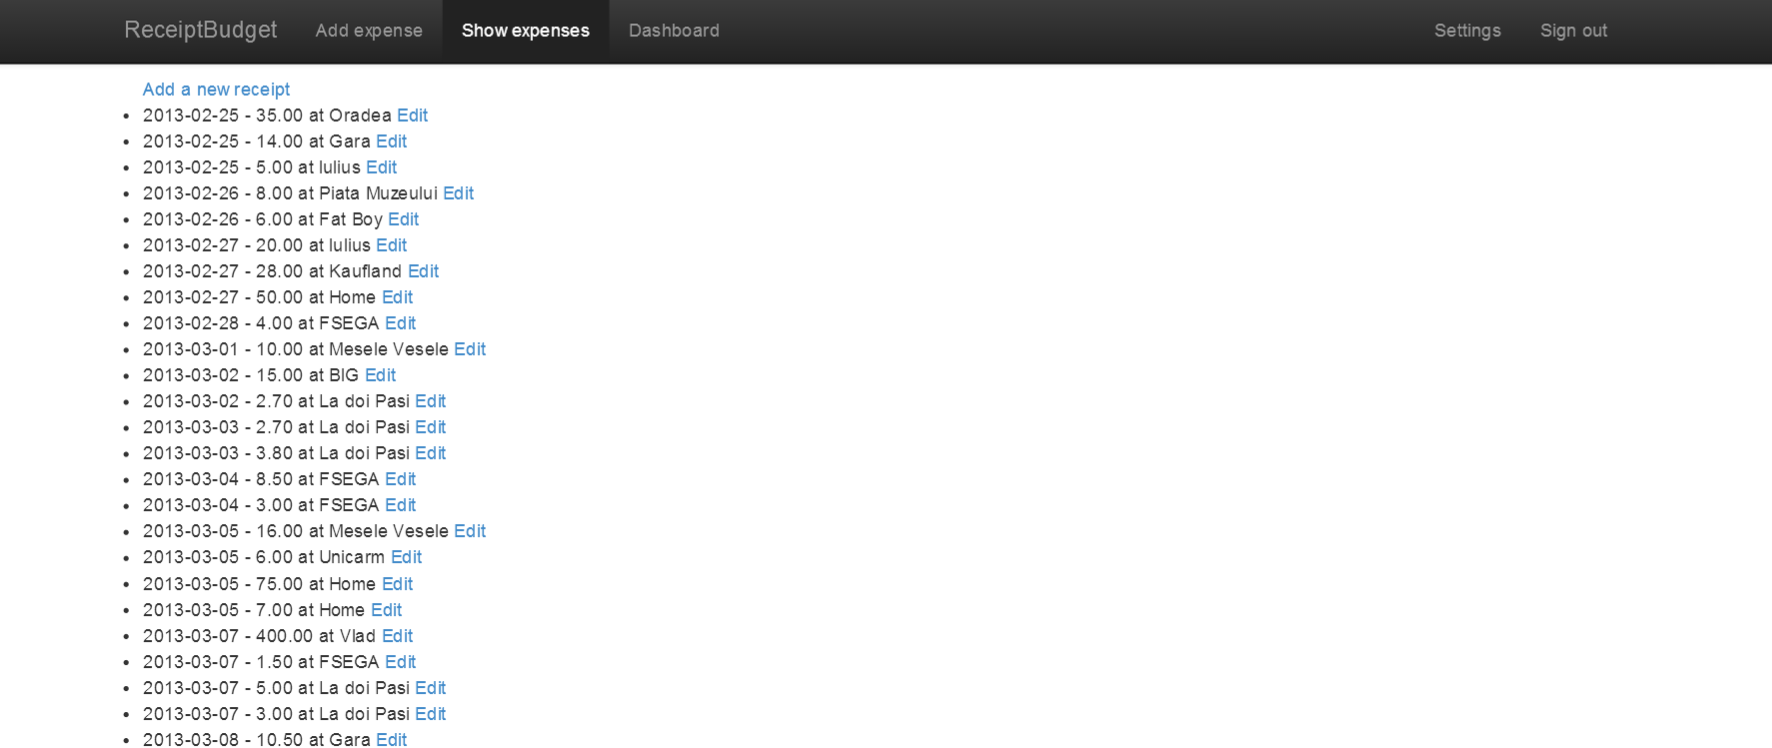
\includegraphics[width=\linewidth]{img/manual/expense_list.png}
\caption{\label{fig:expense_list}
The main page shown to a logged-in user}
\end{center}
\end{figure}

In their user profile (Figure \ref{fig:user_profile}) they can change personal information, such as name, picture and privacy settings (Figure \ref{fig:profile_edit}), their email address or their password.

\begin{figure}[htdp]
\begin{center}
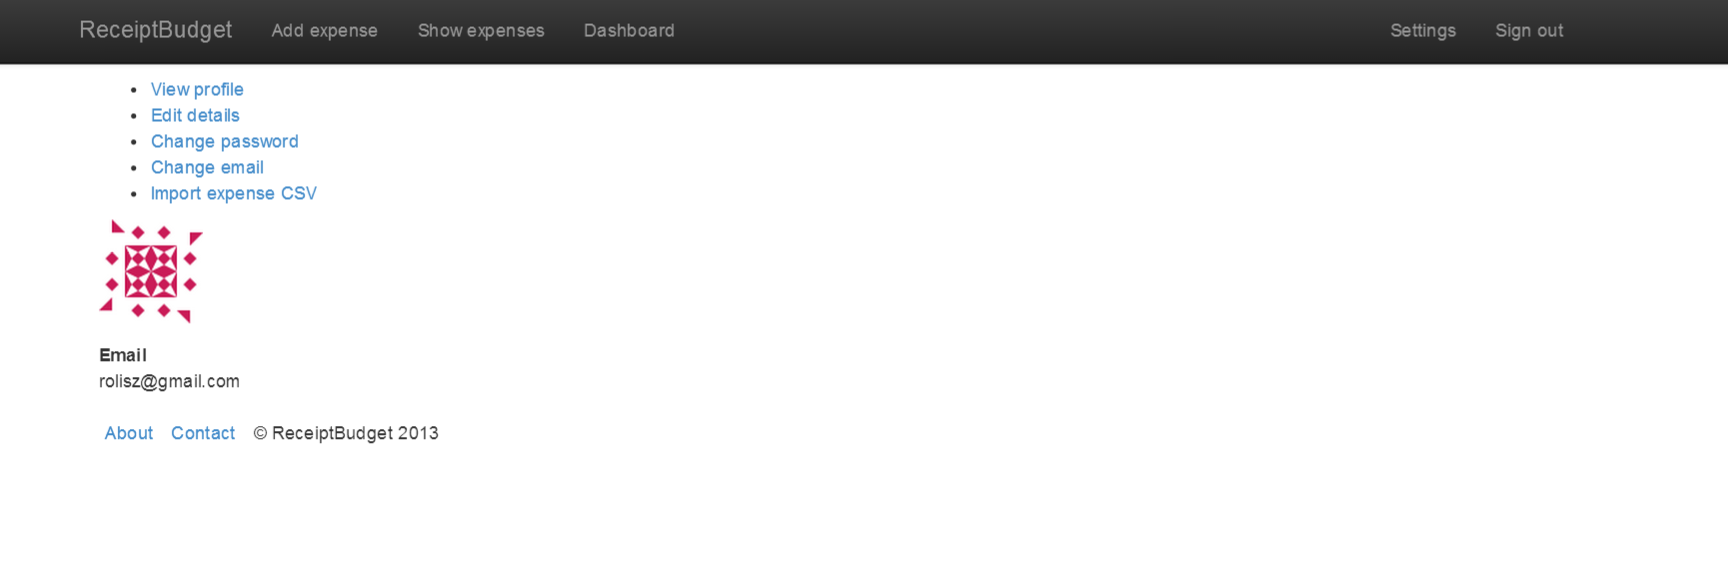
\includegraphics[width=\linewidth]{img/manual/user_profile.png}
\caption{\label{fig:user_profile}
The user profile screen}
\end{center}
\end{figure}

\begin{figure}[htdp]
\begin{center}
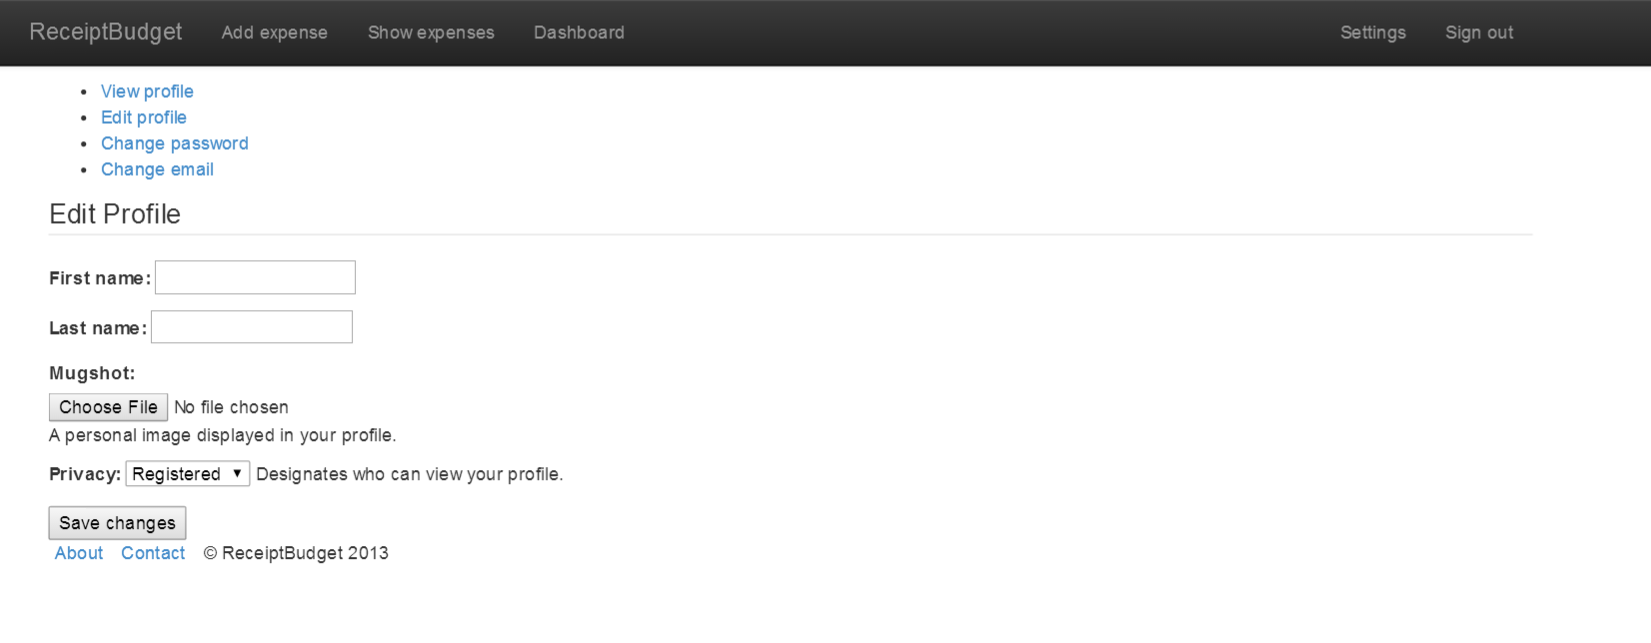
\includegraphics[width=\linewidth]{img/manual/profile_edit.png}
\caption{\label{fig:profile_edit}
The screen for editing the user's own profile}
\end{center}
\end{figure}

On their own personal settings page, the user can import previous expenses that were exported from another personal finance manager in a CSV format. The import tool will try to guess which column from the CSV file corresponds to the internal data structures used by ReceiptBudget and uses heuristics to determine which is the date, expense name, expense value and location where the expense was made. The user has the possibility to correct the guesses made by the application using the screen seen in Figure \ref{fig:csv_import}.

\begin{figure}[htdp]
\begin{center}
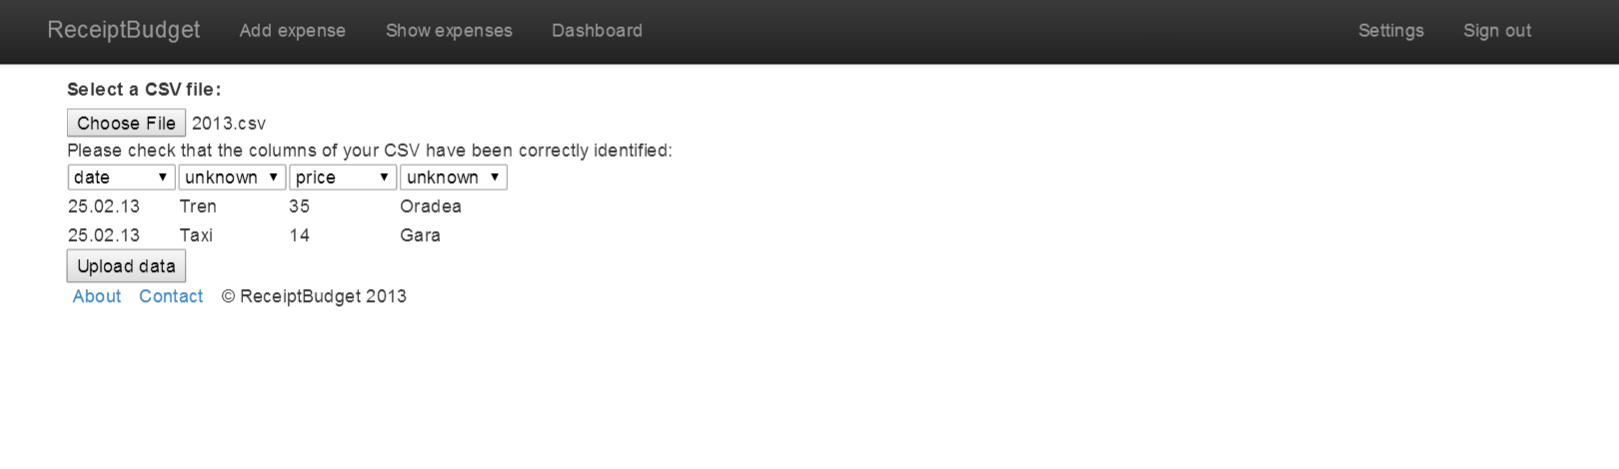
\includegraphics[width=\linewidth]{img/manual/csv_import.png}
\caption{\label{fig:csv_import}
Importing a CSV file containing financial data exported from other programs}
\end{center}
\end{figure}

If a user chooses to add an expense, he has three options. He can add a new expense manually, which is useful for cases where there is no receipt or it was lost, using the form from Figure \ref{fig:manual_add}. Another option would be to add a receipt from an image that is saved on the computer. The last option is to take an image of a receipt with a webcam. In this case the user has to align the receipt and after taking the picture he can select the bounding box for the receipt as seen in Figure \ref{fig:webcam}, and after that he can upload the image to the server. 

\begin{figure}[htdp]
\begin{center}
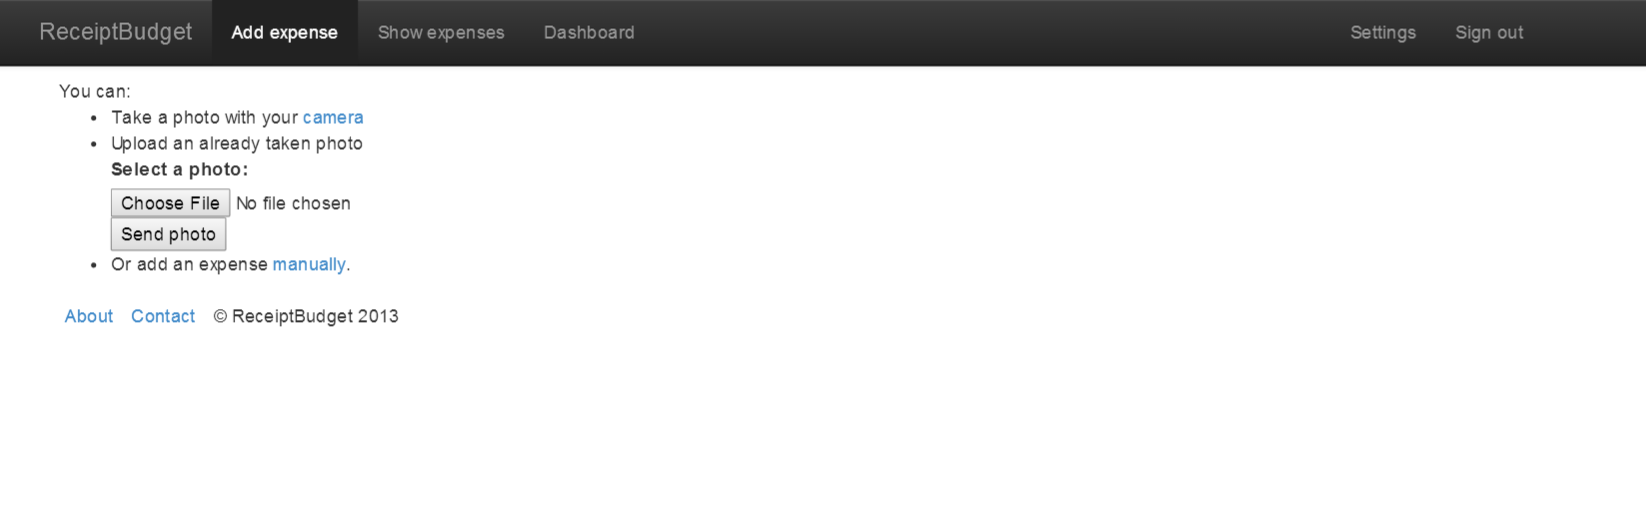
\includegraphics[width=\linewidth]{img/manual/add_expense.png}
\caption{\label{fig:add_expense}
Main screen showing the three options for adding expenses}
\end{center}
\end{figure}

\begin{figure}[htdp]
\begin{center}
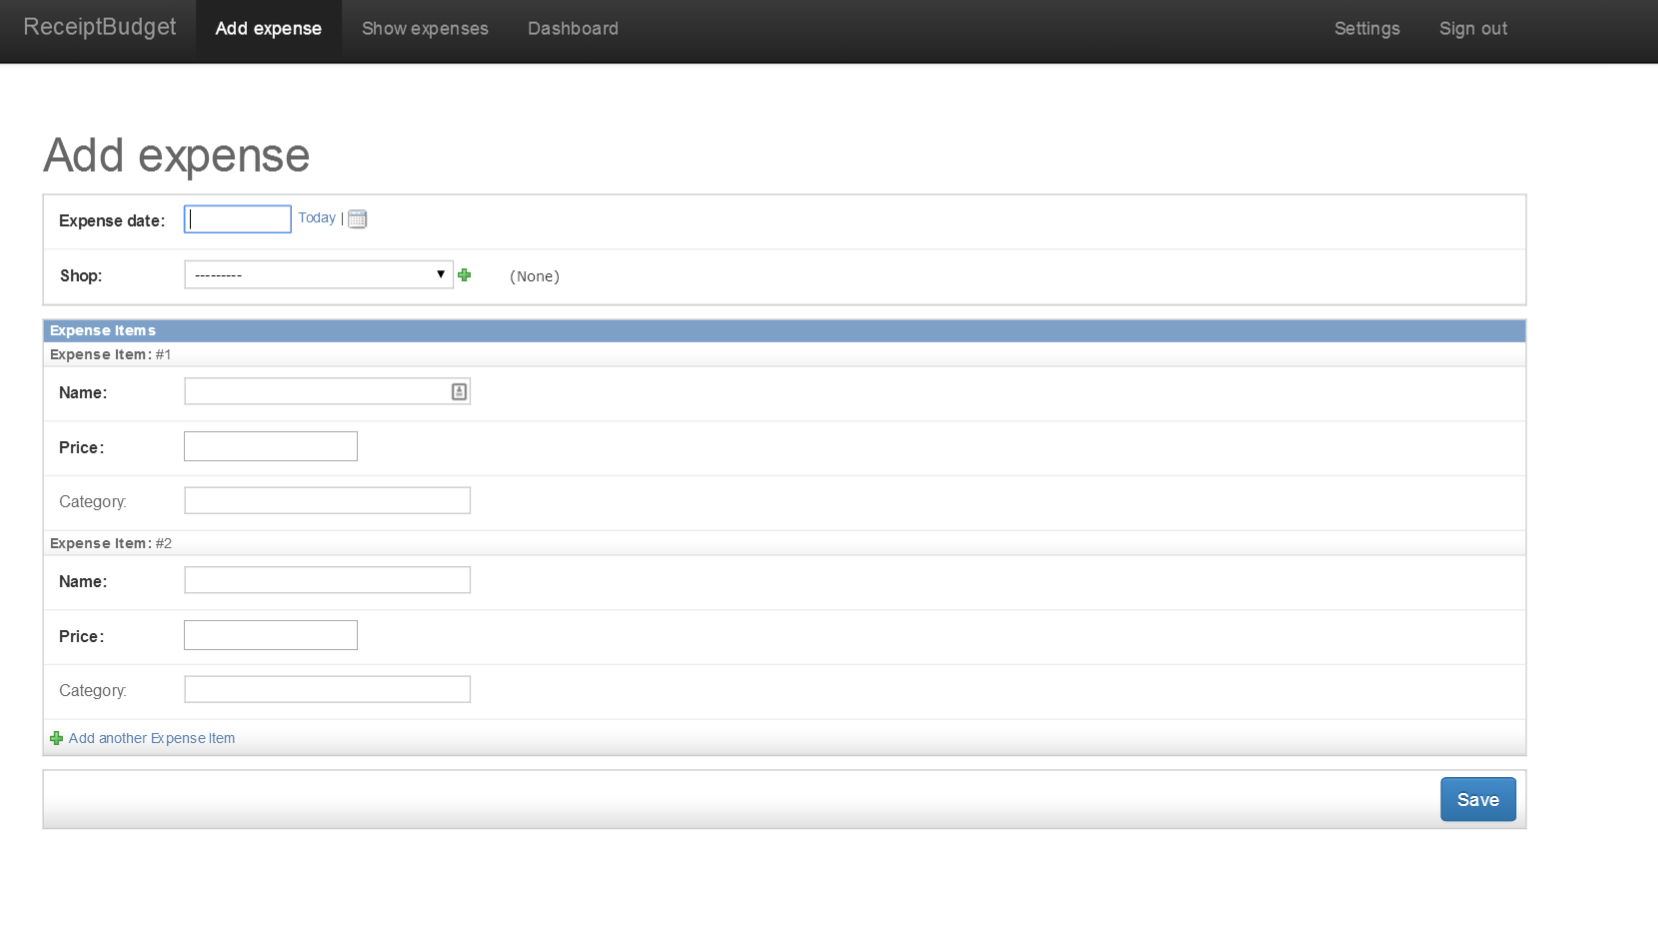
\includegraphics[width=\linewidth]{img/manual/manual_add.png}
\caption{\label{fig:manual_add}
The way to manually add a receipt}
\end{center}
\end{figure}

\begin{figure}[htdp]
\begin{center}
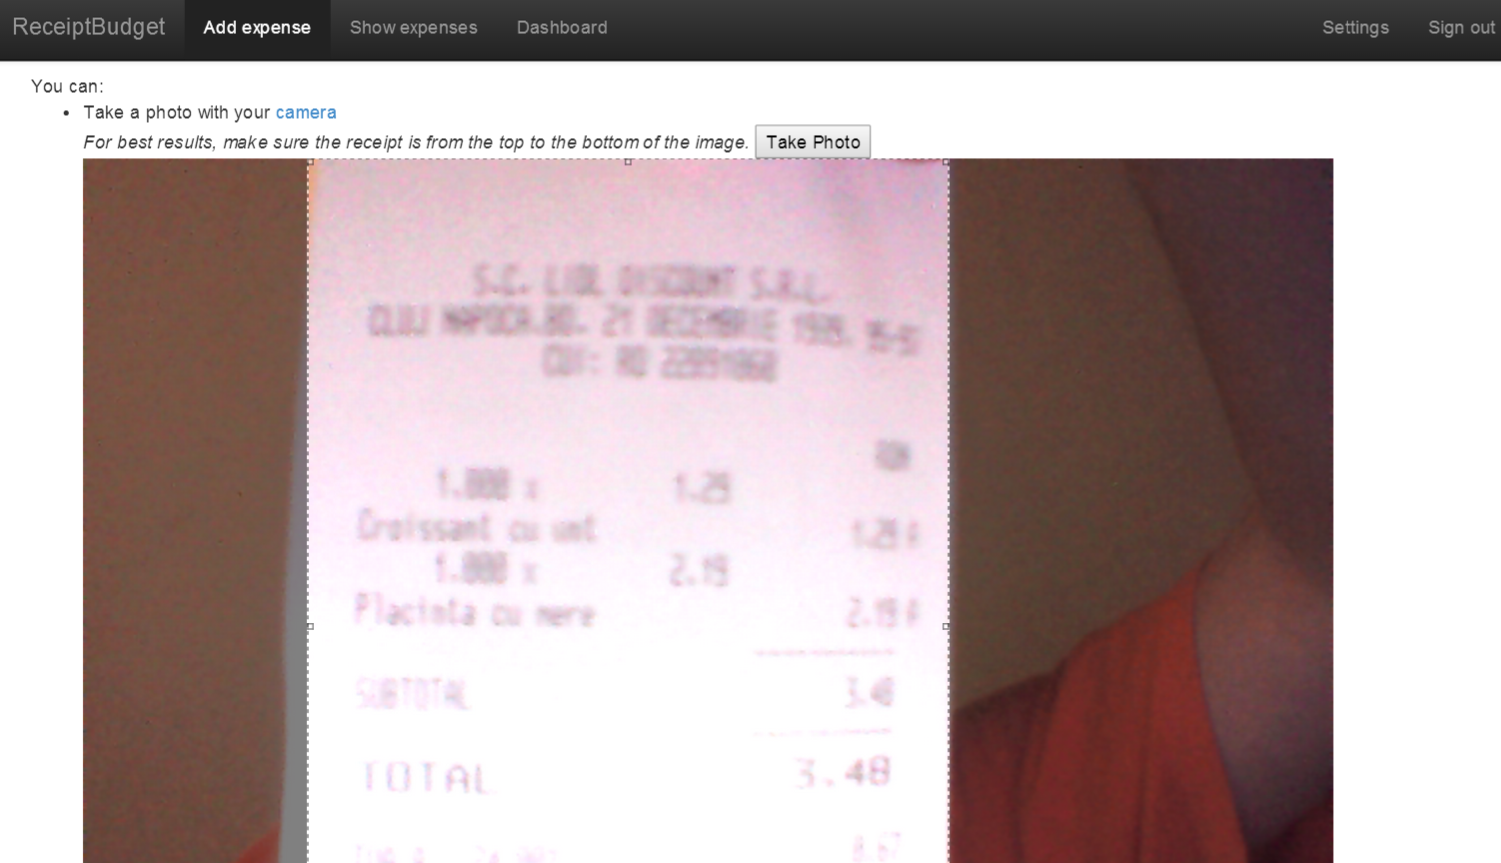
\includegraphics[width=\linewidth]{img/manual/webcam.png}
\caption{\label{fig:webcam}
Adding a receipt by taking a photo with a webcam}
\end{center}
\end{figure}

After the image has uploaded and the OCR engine has returned the extracted information, the user is shown the form from Figure \ref{fig:edit_expense} to edit the results in case there are any errors. After the errors are corrected, the user can save the expenses, or, if he wants, he can choose to discard them. 

\begin{figure}[htdp]
\begin{center}
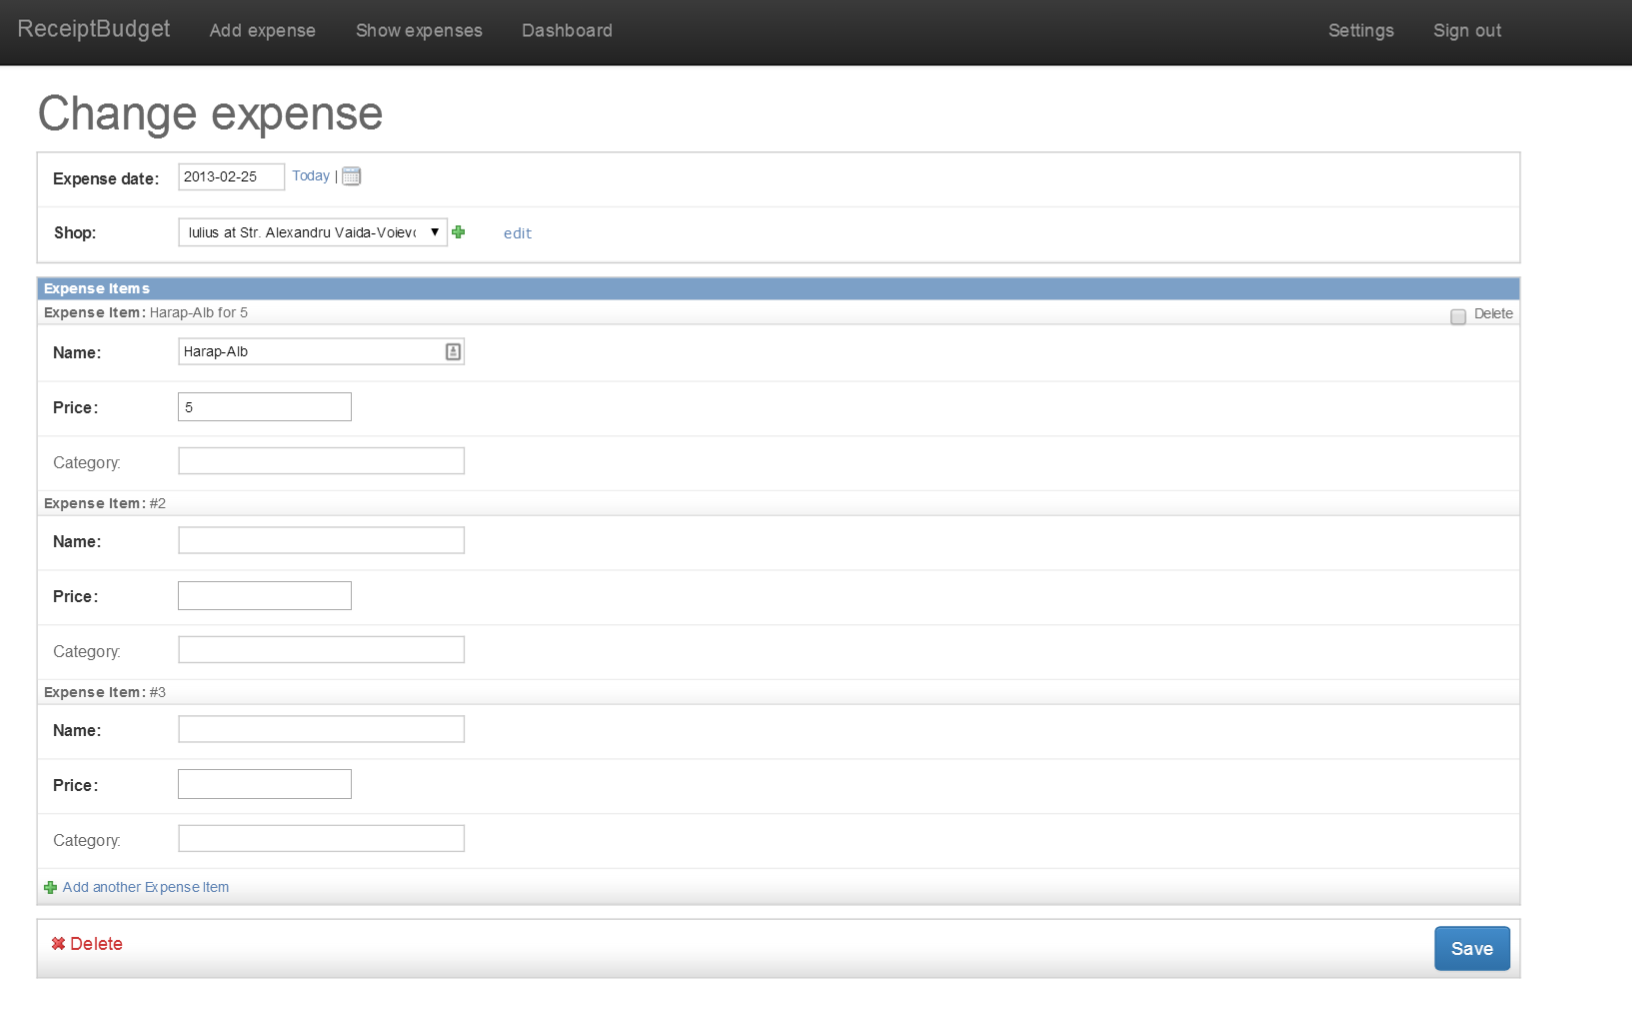
\includegraphics[width=\linewidth]{img/manual/edit_expense.png}
\caption{\label{fig:edit_expense}
Editing a receipt after OCR was performed on it to correct any errors}
\end{center}
\end{figure}

After the user has sufficient expenses in the system, they should visit the dashboard to see their spending pattern. The first visualization they can see on the dashboard is a heat map with all their expenses (Figure \ref{fig:all_map}). The stronger the color red is in an area, the more expenses have been made there. This map can be used to quickly identify hotspots where a lot of expenses are made.

\begin{figure}[htdp]
\begin{center}
\makebox[\textwidth][c]{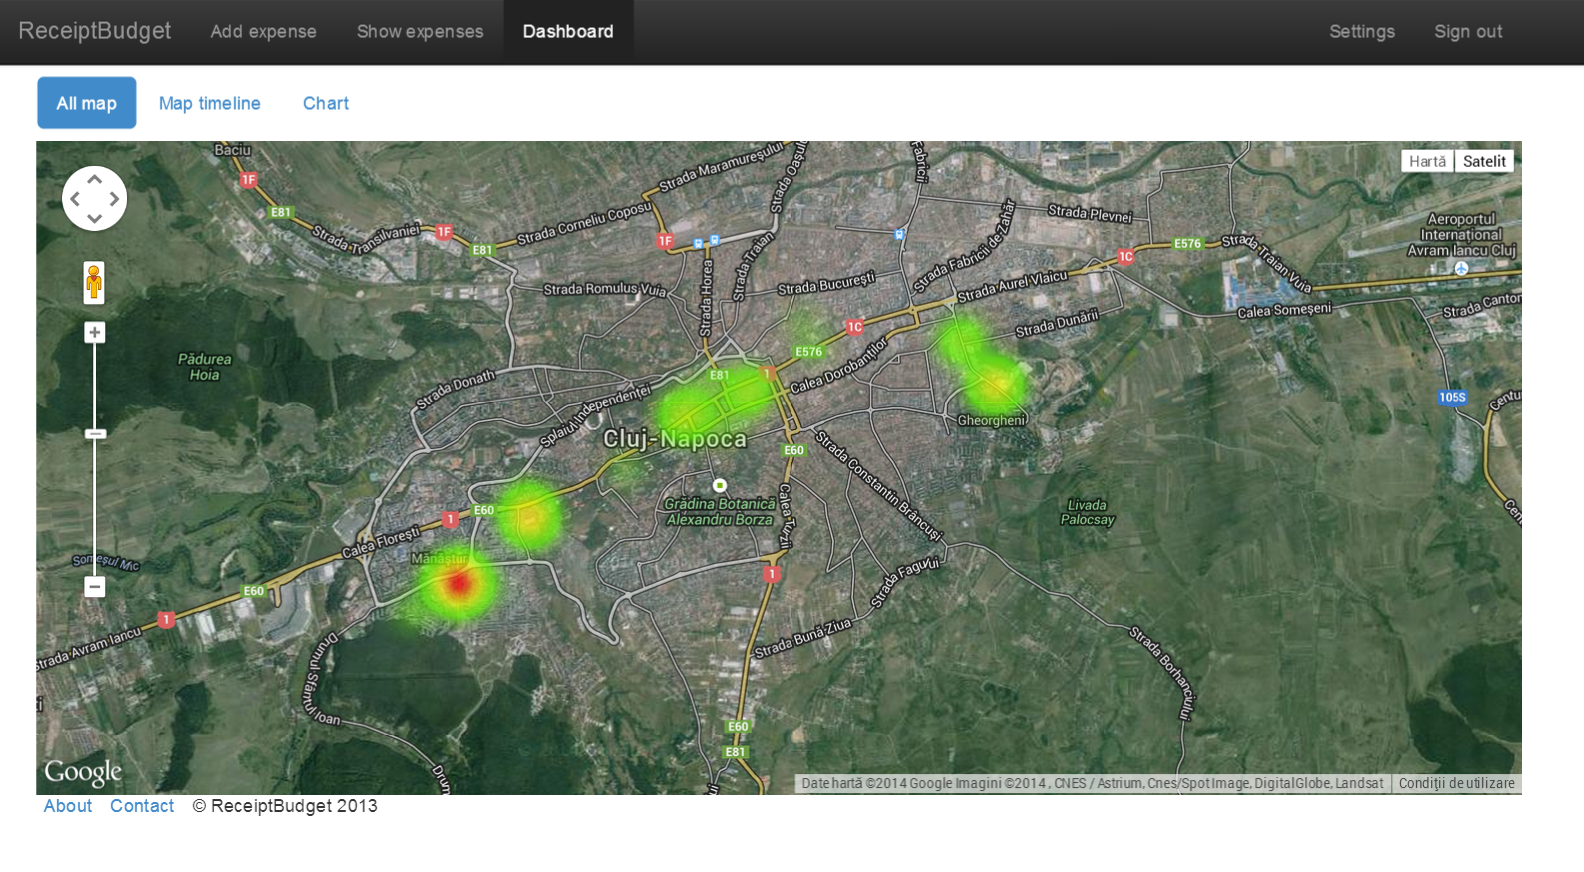
\includegraphics[width=1.2\linewidth]{img/manual/all_map.png}}
\caption{\label{fig:all_map}
The map part of the dashboard showing all expenses made}
\end{center}
\end{figure}

Another visualization is an animation of the way expenses are made each day, also plotted as a heat map (Figure \ref{fig:timeline}). Instead of showing all the expenses at the same time, this visualization breaks them down by day so that the user can see where they spent their money every day. This can be used to detect co-occurring expenses.

\begin{figure}[htdp]
\begin{center}
\makebox[\textwidth][c]{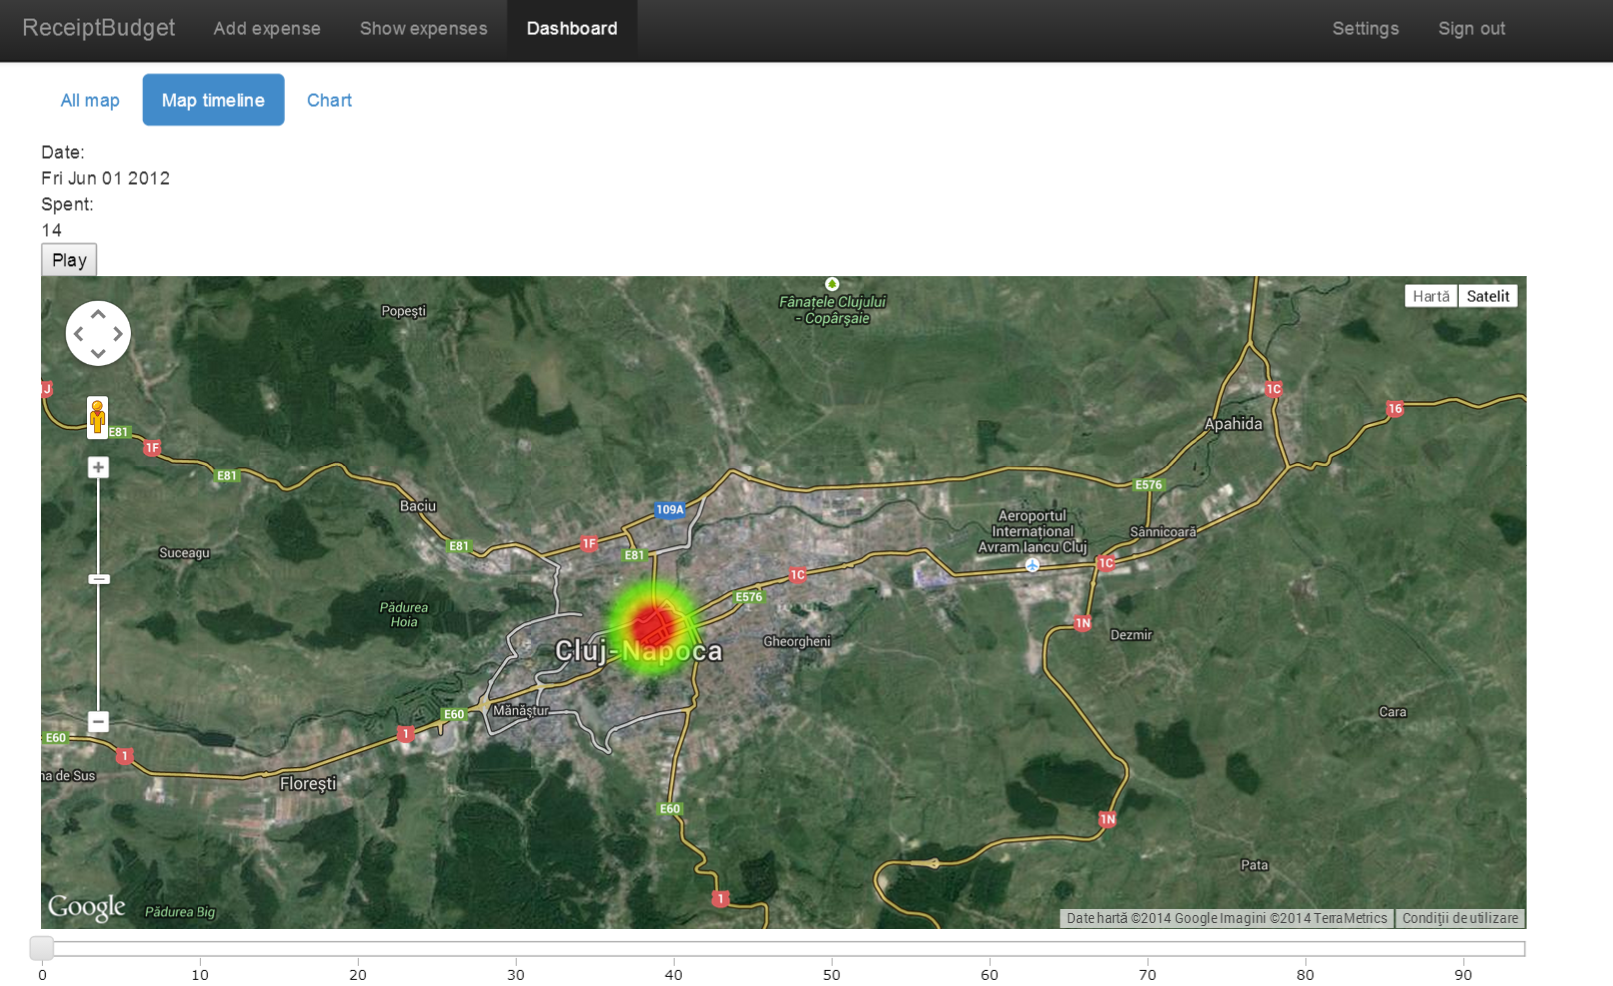
\includegraphics[width=1.2\linewidth]{img/manual/timeline.png}}
\caption{\label{fig:timeline}
A timeline view of the map, showing an animation of how many expenses were made each day}
\end{center}
\end{figure}

The final visualization is the proper dashboard, where there is a pie chart showing what shops was the money spent in, another pie chart showing how much money was spent in each month, a bar chart showing expense breakdown per days of the week, a graph showing the expenses over a range of dates and a table showing the selected expenses (Figures \ref{fig:top_dashboard} and \ref{fig:bottom_dashboard}). This dashboard is interactive and the user can manipulate each chart or graph to select a subset of the data and all the other graphs will be updated so that they show only information from the same subset. In this it is easy to see where a user has spent his money in the months of March, between 2012 and 2014, on weekends. 

\begin{figure}[htdp]
\begin{center}
\makebox[\textwidth][c]{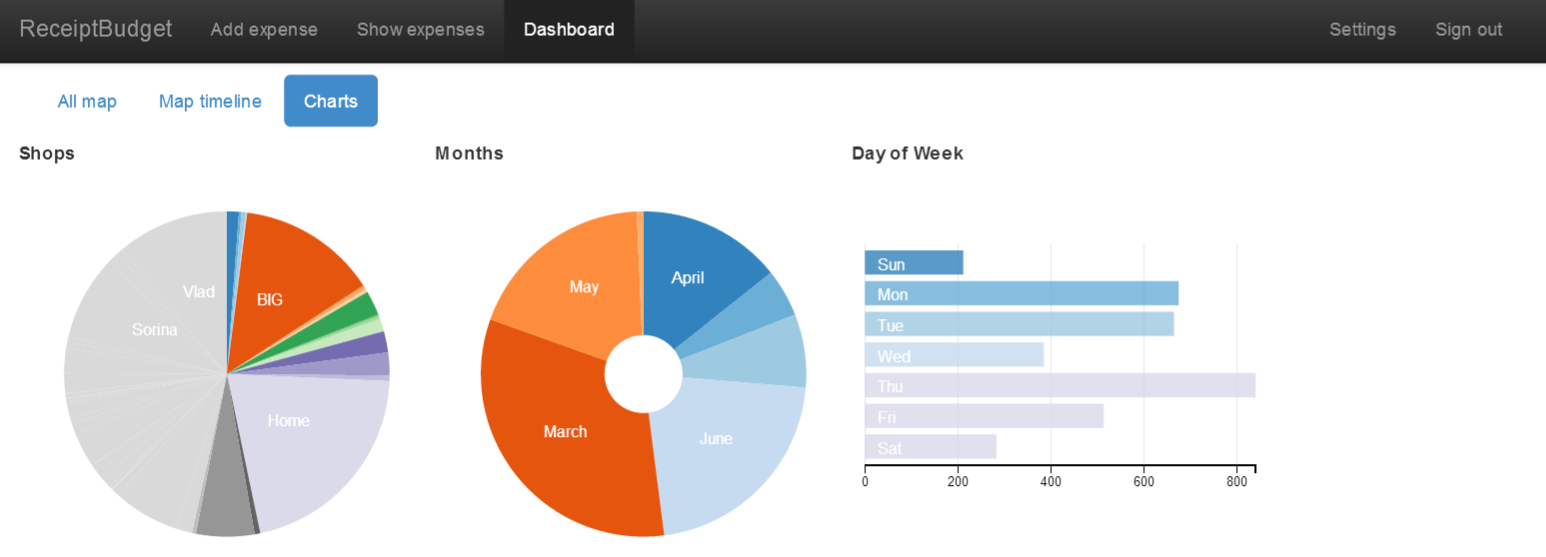
\includegraphics[width=1.2\linewidth]{img/manual/top_dashboard.png}}
\caption{\label{fig:top_dashboard}
The top part of dashboard where the user can filter his expenses}
\end{center}
\end{figure}


\begin{figure}[htdp]
\begin{center}
\makebox[\textwidth][c]{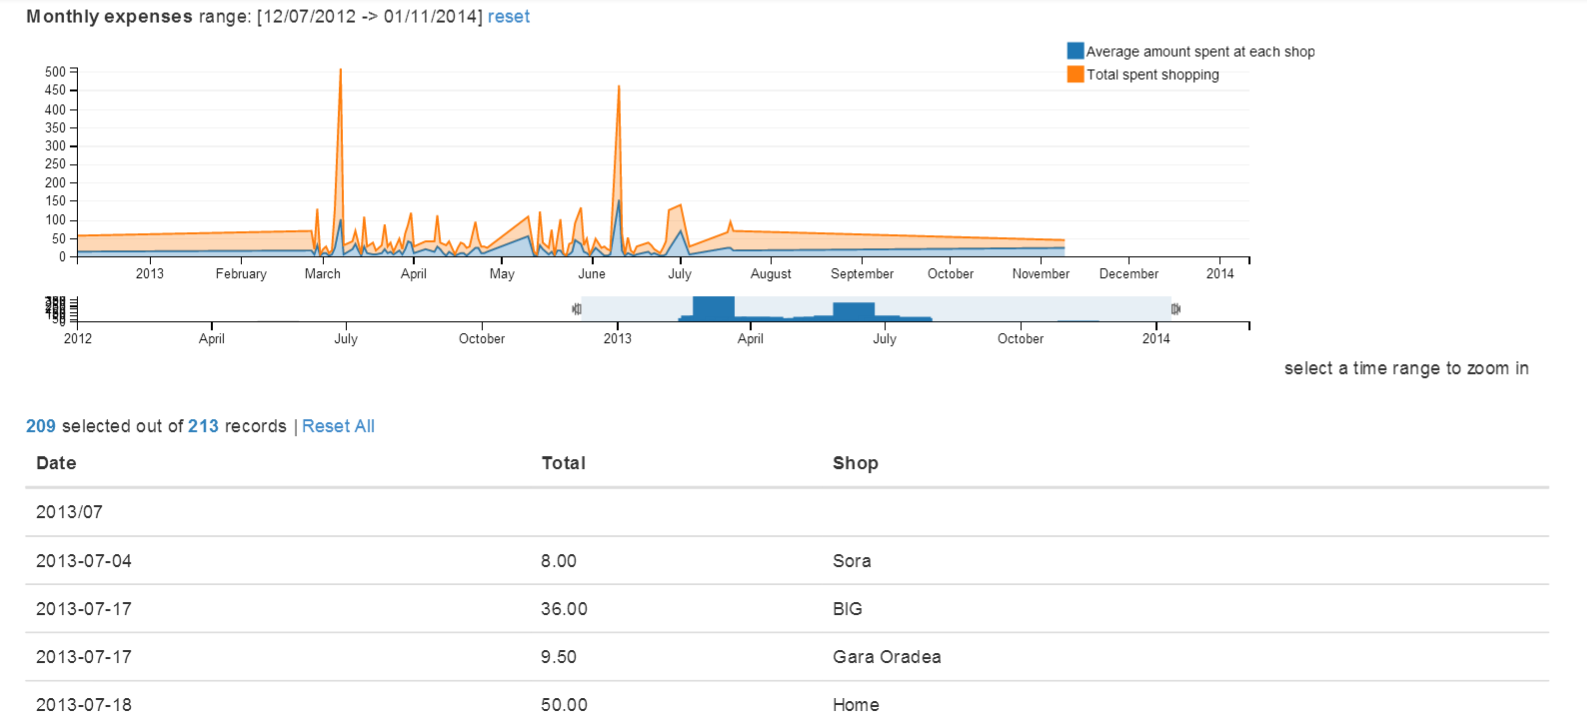
\includegraphics[width=1.2\linewidth]{img/manual/bottom_dashboard.png}}
\caption{\label{fig:bottom_dashboard}
The lower part of the dashboard}
\end{center}
\end{figure}